\section{Architettura}

Il nostro progetto contiene tre progetti distinti:

\begin{enumerate}
	\item La libreria effettiva (cartella \path{lib/})
	\item Una piccola applicazione a riga di comando (cartella \path{cli/})
	\item Un'applicazione a interfaccia grafica (cartella \path{QTInterface/})
\end{enumerate}

La libreria viene compilata producendo in output un file binario non eseguibile; per poterla utilizzare, gli altri due sottoprogetti (indipendenti tra loro) vengono linkati con esso per poter produrre un file eseguibile. Questa struttura permette di scindere in modo netto il codice dei nostri applicativi "client" da quello della libreria, incentivando al riutilizzo in contesti diversi.

\subsection{Libreria effettiva}
Come citato in precedenza, questo è il sottoprogetto principale tra quelli presenti. Il componente più importante è la classe \texttt{IterativeSolver}. Questa classe estende (e implementa, essendo concreta) la classe astratta \texttt{Solver}. All'interno di questa classe e della sua superclasse  è presente un metodo \texttt{solve} che prende in input la matrice dei coefficienti, il vettore dei termini noti e restituisce il vettore soluzione calcolato. Il punto fondamentale della risoluzione di un sistema in modo iterativo è il ciclo che esegue gli update a partire dalla soluzione corrente: essendo uguale per qualsiasi metodo, abbiamo fatto in modo che il solver iterativo avesse come attributo di istanza un tipo astratto di regola di update, che viene estesa e implementata dalle regole specifiche istanzate da chi usa la libreria. questa è l'applicazione del design pattern \textit{Strategy} \cite{Strategy}. Esiste una classe concreta per ognuno dei quattro metodi richiesti.

La classe generica di update (\path{UpdateStrategy}) dichiara due metodi principali: \path{init}, che viene chiamato dal solver prima di cominciare le iterazioni, e \path{update}, che viene usato per creare la nuova soluzione all'interno del ciclo di esecuzione del solver.

\subsection{Applicazione da riga di comando}
Questo sottoprogetto è molto piccolo: contiene principalmente il metodo main, che legge gli argomenti passati come input, e un file header, \path{runner.h}, che contiene il codice che chiama la libreria solver. Questo header è lo stesso che viene chiamato dall'interfaccia grafica; pertanto, si trova nella cartella principale, piuttosto che nella sottocartella \path{cli/}.


\subsection{Applicazione GUI}
Abbiamo creato anche una piccola applicazione con interfaccia grafica usando il framework Qt \cite{Qt}. Questa permette di:
\begin{itemize}
	\item Selezionare il file contenente la matrice de coefficienti
	\item Regolare i parametri $\omega$ per i metodi di Jacobi e Gauss-Seidel;
	\item Selezionare il tipo di norma da calcolare in fase di controllo della convergenza. Le scelte possibili sono euclidea, manhattan e infinito;
	\item Decidere di saltare il controllo che stabilisce se la matrice è simmetrica e definita positiva\footnote{Questa opzione può tornare utlie per eventuali benchmark. Infatti, questo controllo richiede diverso tempo e rischia di nascondere le differenze tra i vari metodi in termini di tempo, sopratttutto per matrici relativamente piccole};
	\item Visualizzare i risultati dei metodi sotto forma di tabella e di grafici che mostrano l'errore relativo e i tempi in funzione della tolleranza, ragruppati per metodo (Figura \ref{fig:ui:output}).
	\item Esportare i risultati in formato CSV.
\end{itemize}

\begin{figure}%
	\centering
	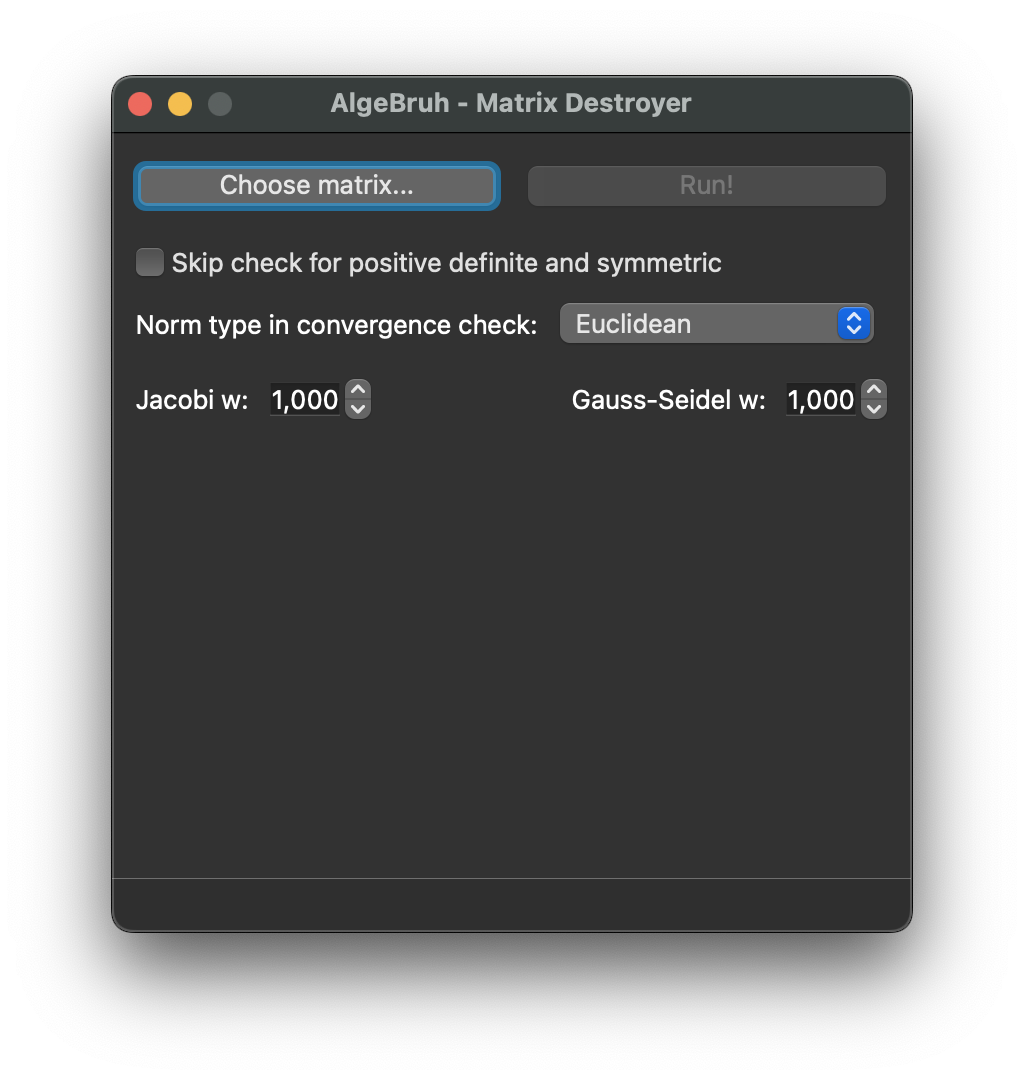
\includegraphics[width=0.5\textwidth]{figures/UI/main.png}
	\caption{Schermata iniziale dell'applicazione}%
	\label{fig:ui:main}%
\end{figure}

\begin{figure}%
	\centering
	\subfloat[\centering  Tabella riassuntiva]{{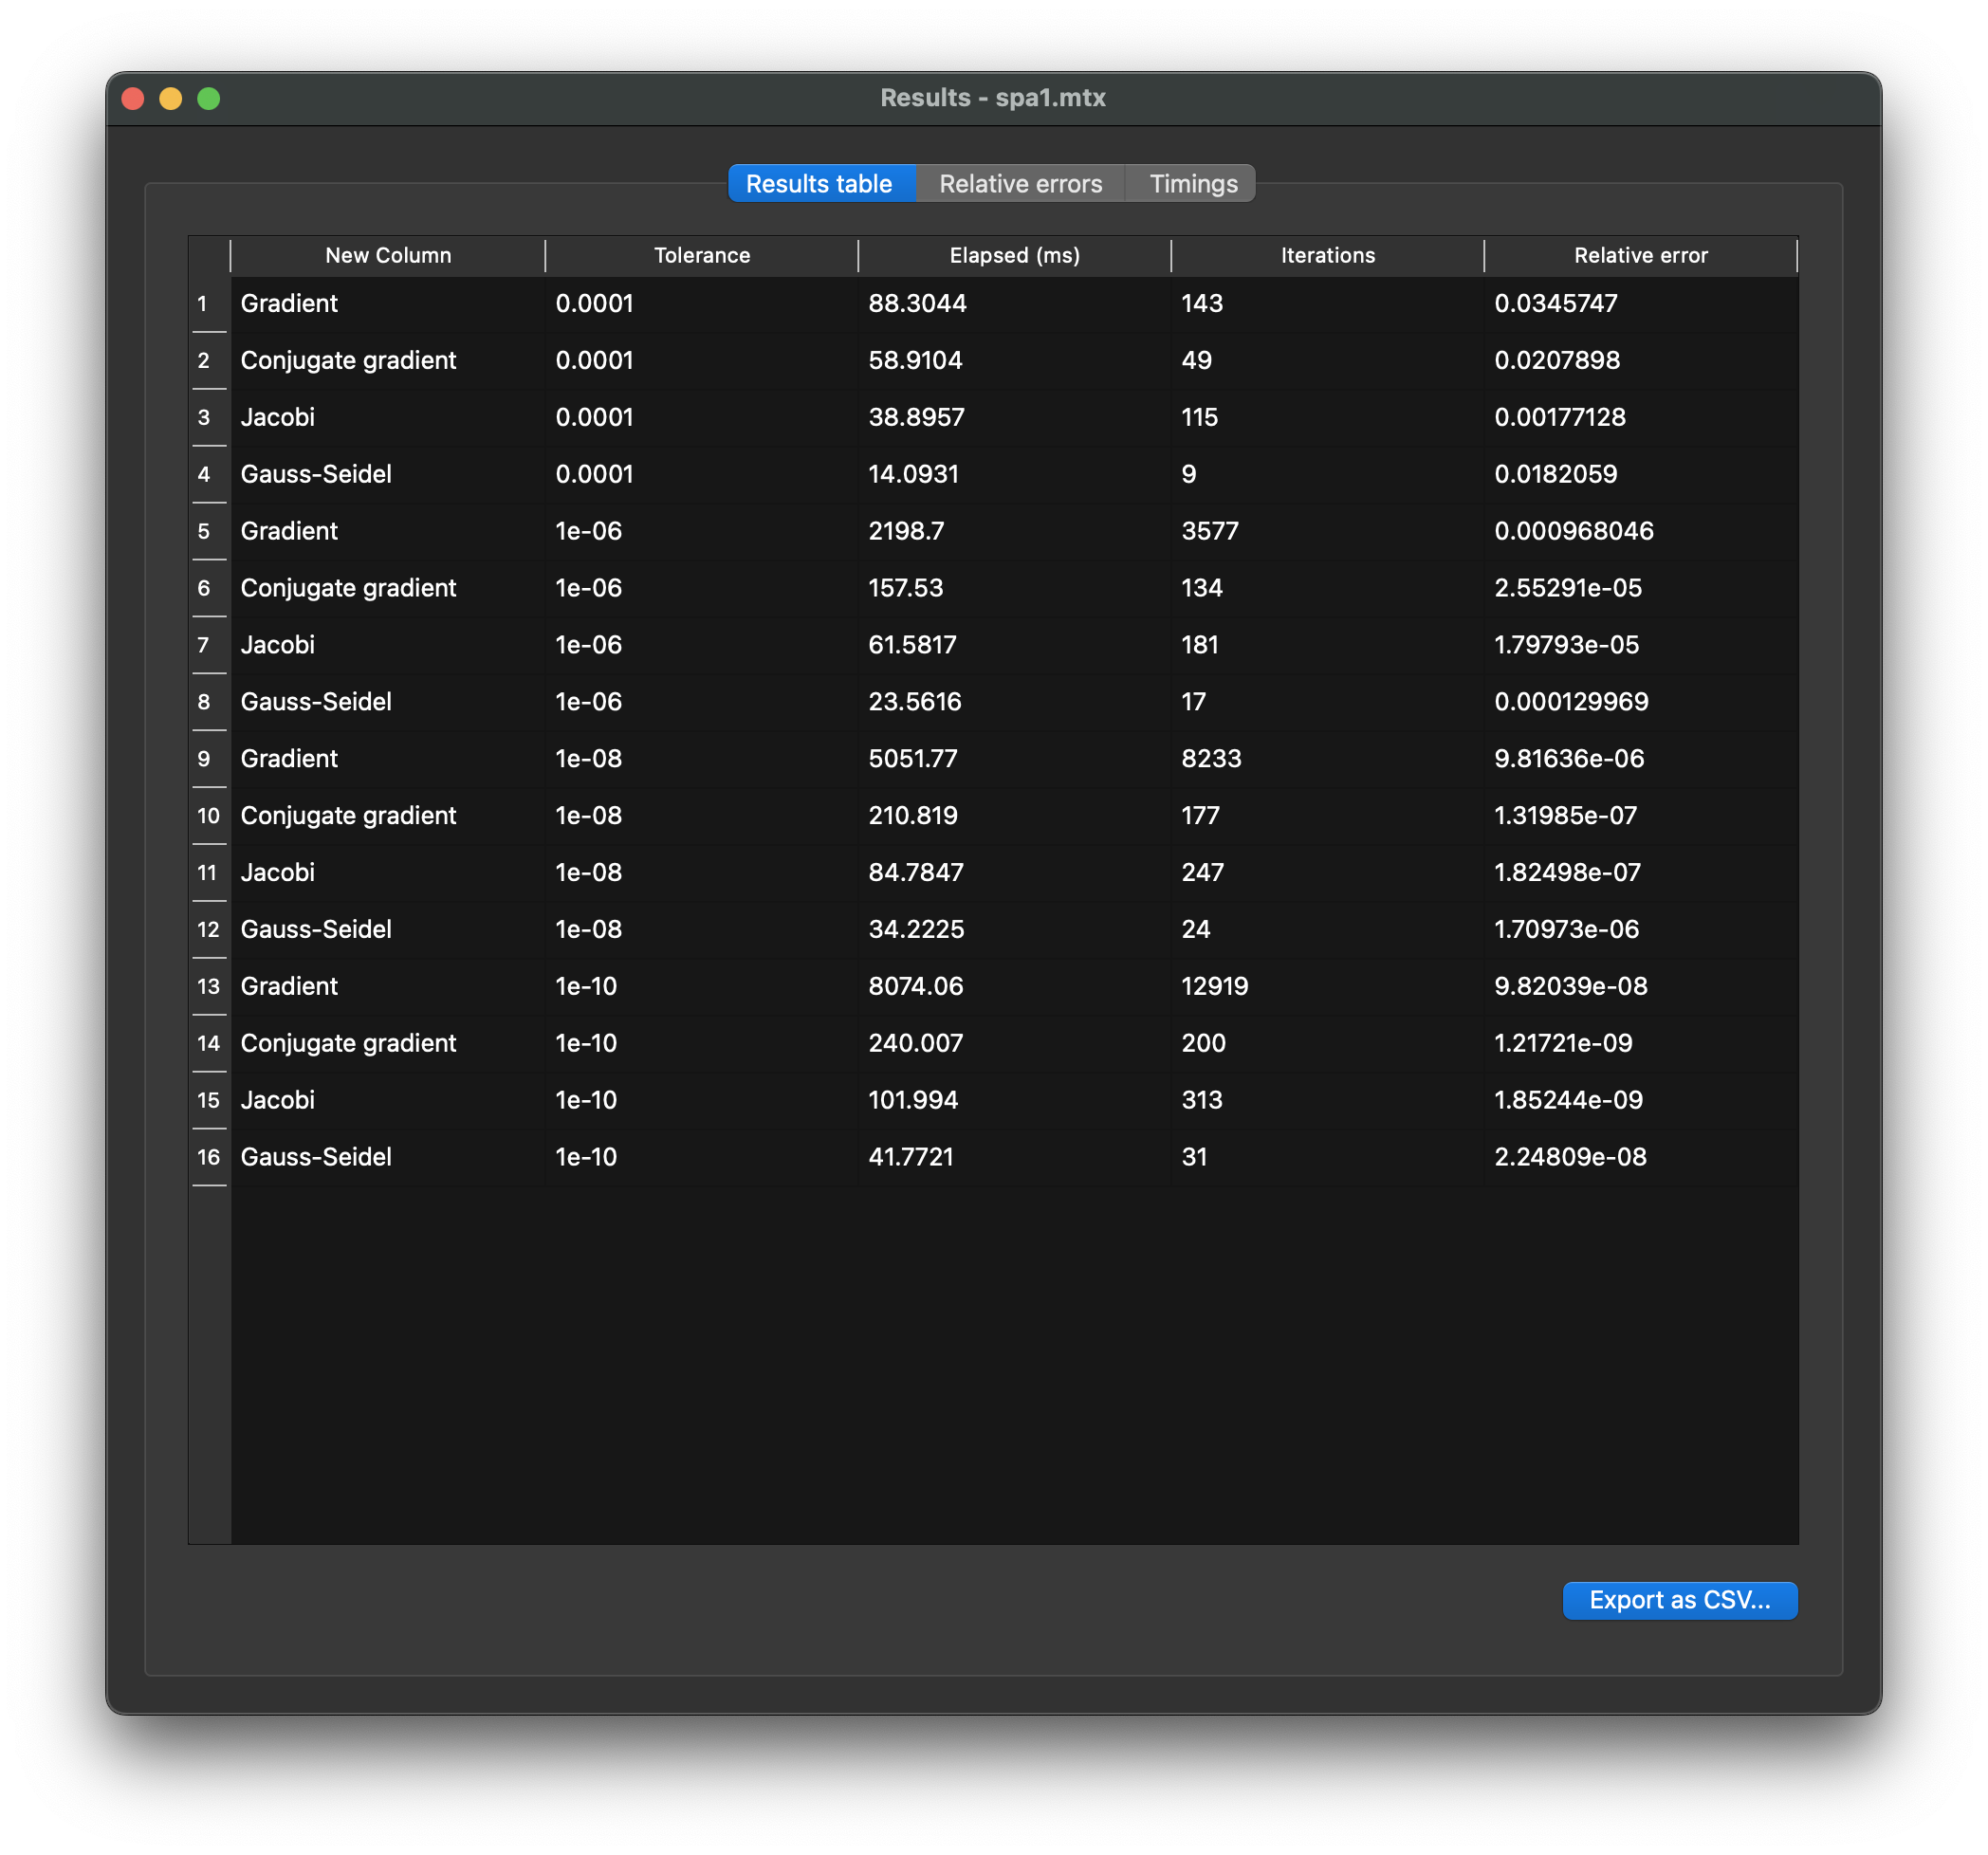
\includegraphics[width=0.45\textwidth]{figures/UI/table} }}%
	\qquad
	\subfloat[\centering Grafico tolleranza / tempi]{{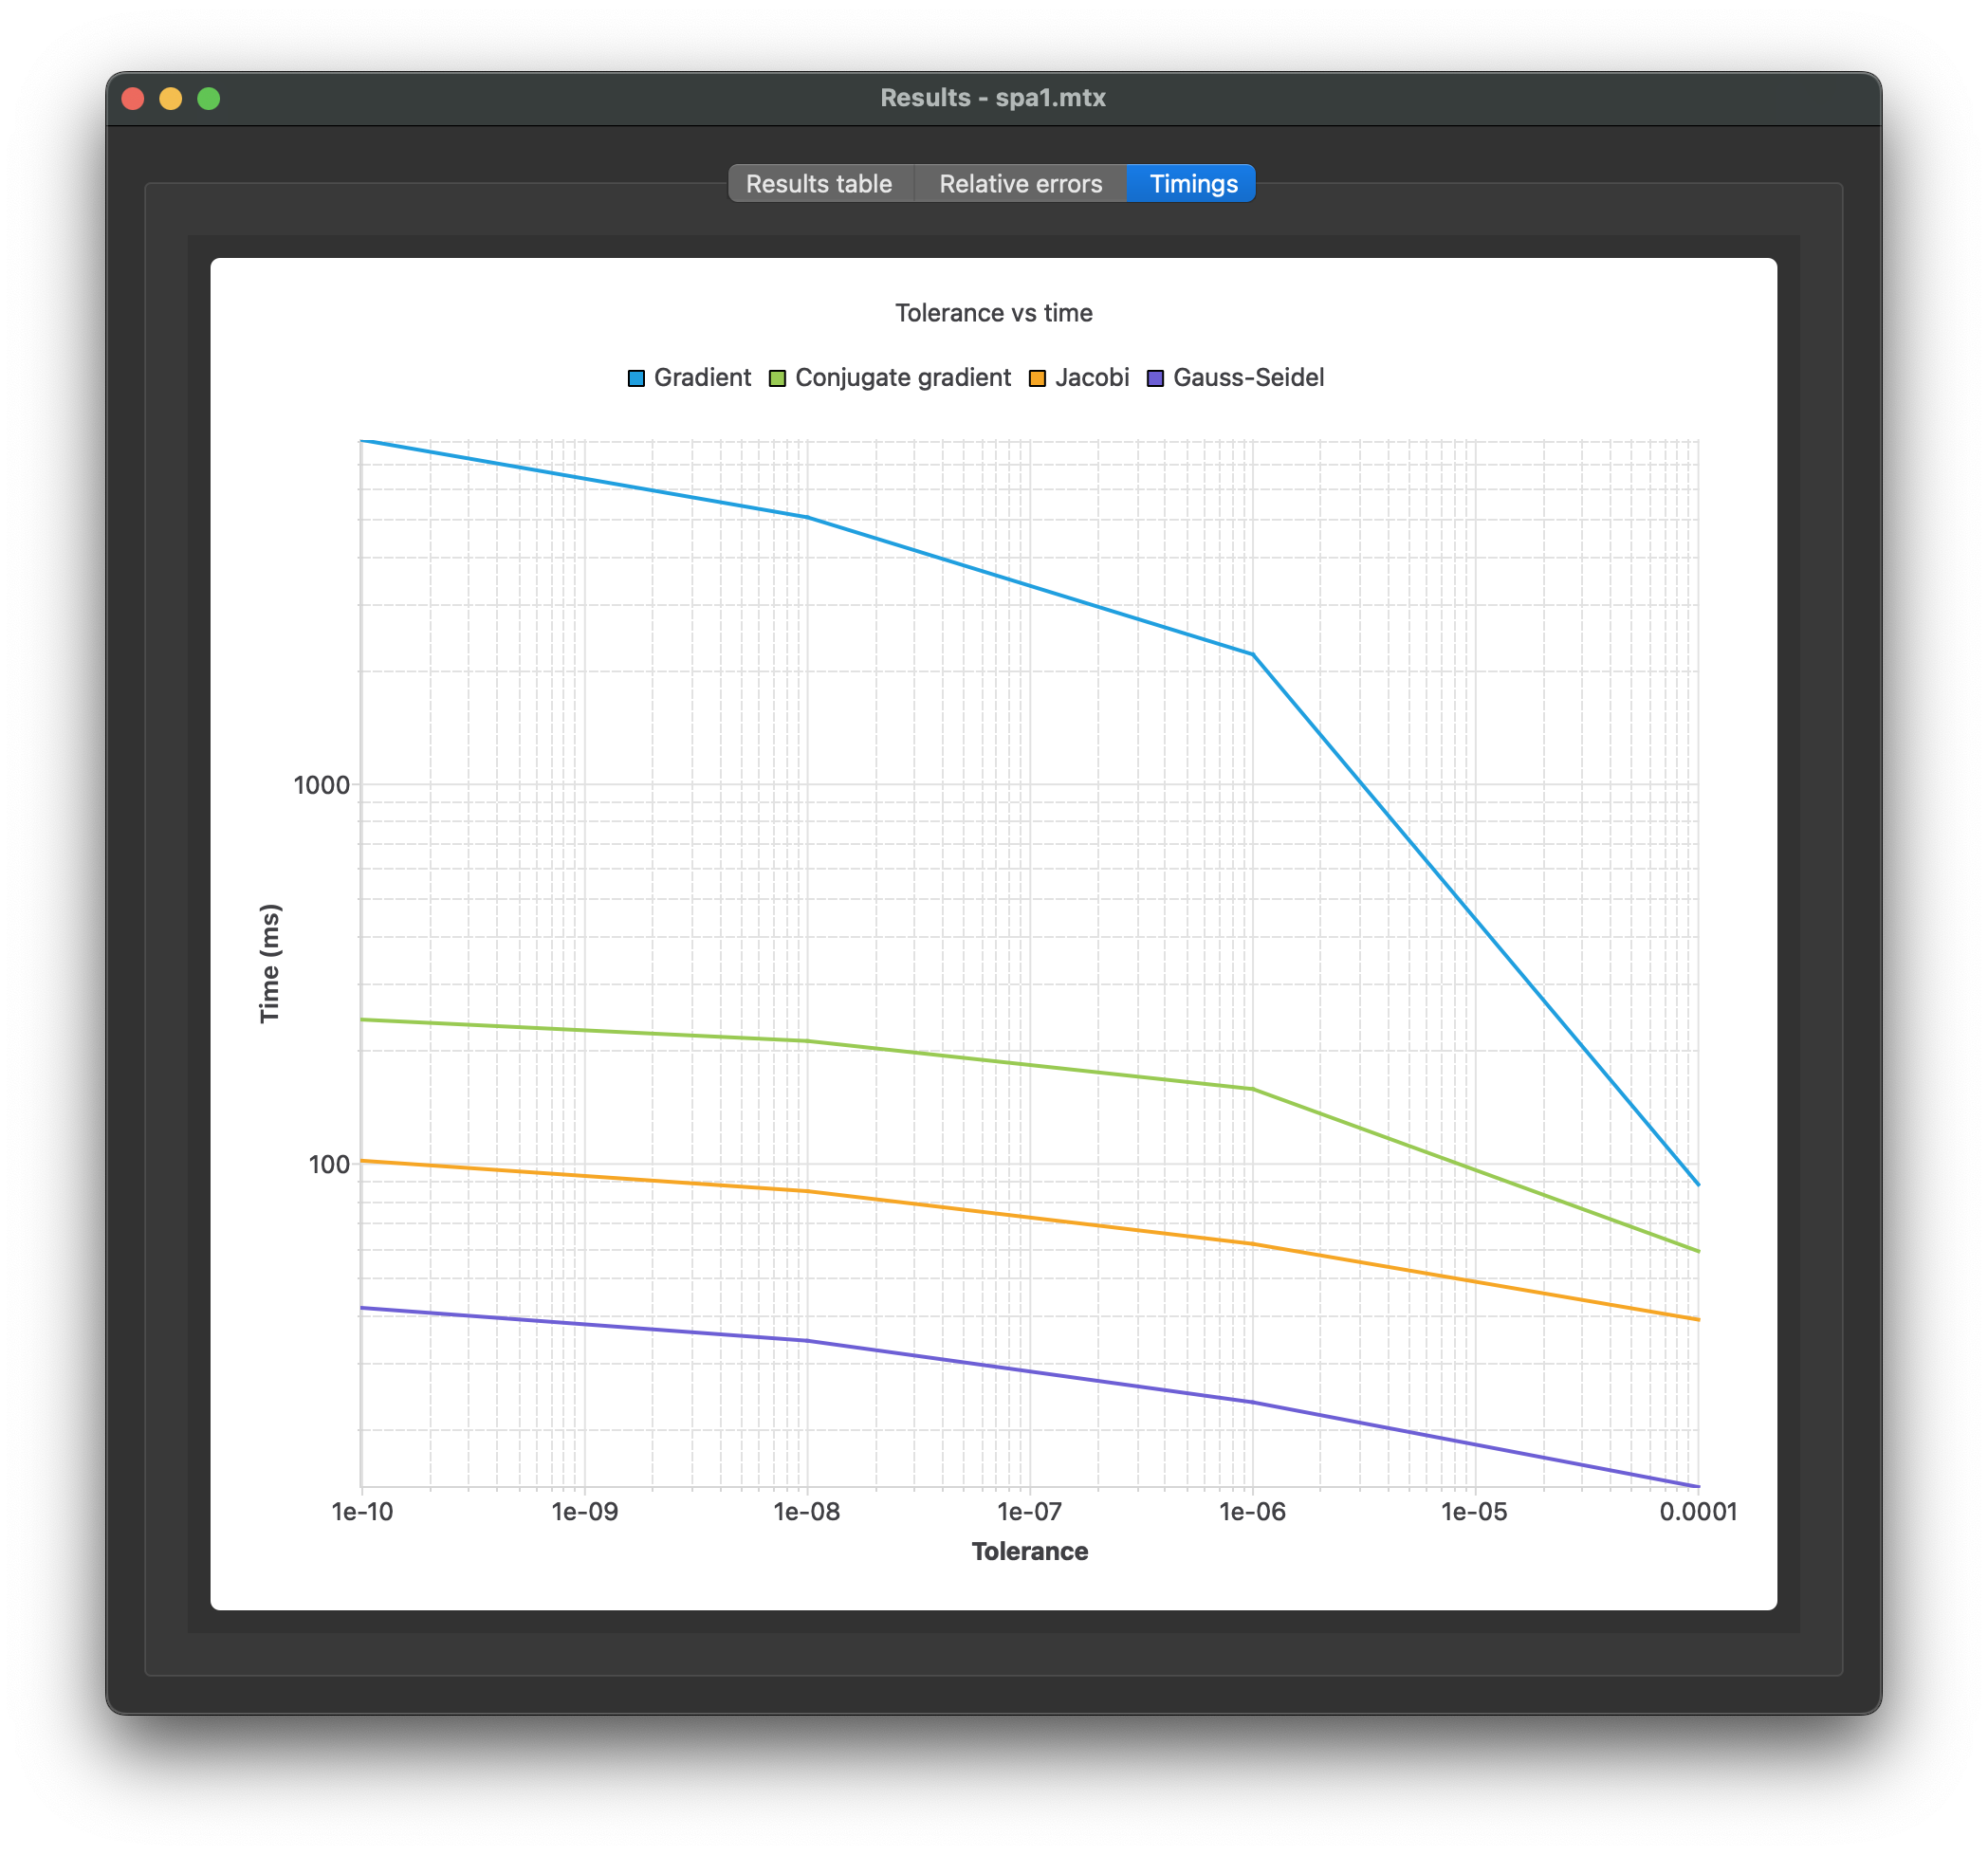
\includegraphics[width=0.45\textwidth]{figures/UI/chart} }}%
	\caption{Esempi di output prodotti dall'applicazione Qt}%
	\label{fig:ui:output}%
\end{figure}

Come per il progetto da riga di comando, questo è un eseguibile che effettua un linking statico verso la libreria, restando dunque un progetto separato da un punto di vista logico.